
\lecture{Confidence Intervals}{confidence-interval}
\section{Confidence Intervals}

\title{The Confidence Interval}
\subtitle{Introducing the Idea}

%\author{Kelly Black}
%\institute{Clarkson University}
\date{29 February 2012}

\begin{frame}
  \titlepage
\end{frame}

\begin{frame}
  \frametitle{Outline}
  \tableofcontents[pausesection,hideothersubsections,sectionstyle=show/hide]
\end{frame}


\subsection{Clicker Quiz}


\begin{frame}
  \frametitle{Clicker Quiz}

  You sample a random variable which has a mean of 2.1 and a standard
  deviation of 4.5. You take 30 samples. What is the probability that
  the sample mean is more than 3.5?

  \vfill

  \begin{tabular}{l@{\hspace{3em}}l@{\hspace{3em}}l@{\hspace{3em}}l}
    A: 0.0446  & B: 0.6221  & C: 0.9954
  \end{tabular}

  \vfill
  \vfill
  \vfill

\end{frame}

\subsection{The Confidence Interval}


\begin{frame}
  \frametitle{Problem!}

  We have a random variable. It has a mean, $\mu$, and a standard
  deviation, $\sigma$. How do we know?

  \vfill

  \only<2->
  {
    \begin{block}{Example}
      We run a capitol investment firm. Someone asks us for \$250,000
      to start a restaurant. It this a reasonable amount?
    \end{block}
  }

  \vfill

\end{frame}


\begin{frame}{The Big Question}

  How do we estimate the mean of a random variable?
  
\end{frame}


\begin{frame}{Example}
  
  We call up ten restaurant owners and ask them for the amount they
  needed to get started. We then calculate a \textit{sample mean},
  \begin{eqnarray*}
    \bar{x} & = & \frac{x_1 + x_2 + x_3 + x_4 + x_5 + x_6 + x_7 + x_8 + x_9 + x_{10}}{10}.
  \end{eqnarray*}
  This is our \textbf{estimate} for the mean.
  
\end{frame}


\begin{frame}
  \frametitle{Clicker Quiz}

  We call up ten restaurant owners and ask them for the amount they
  needed to get started. We then calculate a \textit{sample mean},
  \begin{eqnarray*}
    \bar{x} & = & \frac{x_1 + x_2 + x_3 + x_4 + x_5 + x_6 + x_7 + x_8 + x_9 + x_{10}}{10}.
  \end{eqnarray*}

  Is this estimate close to the true mean?

  \vfill

  \begin{tabular}{l@{\hspace{3em}}l@{\hspace{3em}}l@{\hspace{3em}}l}
    A: Yes  & B: No  & C: Maybe??
  \end{tabular}

  \vfill
  \vfill
  \vfill

  *
\end{frame}


\begin{frame}{Estimators}

  \begin{definition}{Bias}
    \begin{itemize}
    \item If our estimator for a parameter is expected to be less that
      the true value is has a \textit{negative bias.}
    \item If our estimator for a parameter is expected to be more that
      the true value is has a \textit{positive bias.}
    \item If the expectation of our estimator for a parameter is the
      same as the true value then it is \textit{unbiased.}
    \end{itemize}
  \end{definition}
  
  \vfill

\end{frame}


\begin{frame}{Estimator - An example}

  \begin{definition}{Estimator of the mean}
    The sample mean is an estimator of the mean,
  \begin{eqnarray*}
    \bar{x} & = & \frac{x_1 + x_2 + x_3 + \cdots + x_{n}}{n}.
  \end{eqnarray*}    
  \end{definition}
  
  \vfill
  \vfill
  \vfill

  *
\end{frame}



\begin{frame}
  \frametitle{Estimator for the mean}


  \only<1>{\centerline{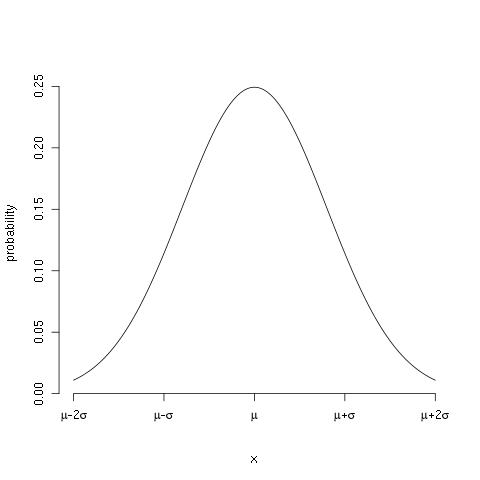
\includegraphics[width=6cm]{img/week8Dist}}}
  \only<2>{\centerline{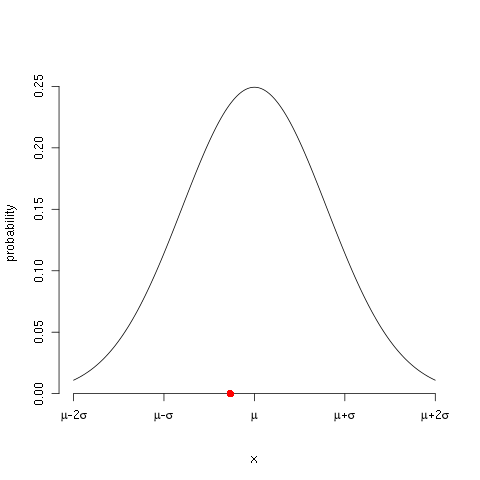
\includegraphics[width=6cm]{img/week8DistSample}}}
  \only<3>{\centerline{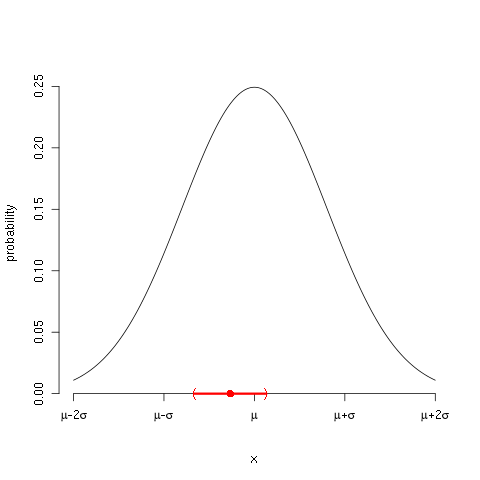
\includegraphics[width=6cm]{img/week8DistConfInterval}}}

\end{frame}



\begin{frame}
  \frametitle{Clicker Quiz}


  \centerline{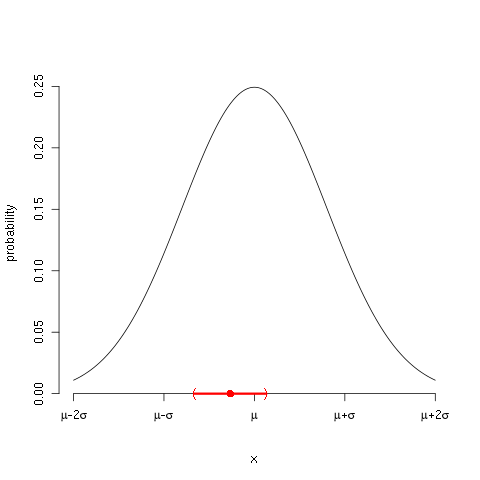
\includegraphics[width=6cm]{img/week8DistConfInterval}}
  If the value of $\alpha$ is increased does the length of the
  ``error'' increase or decrease?  \vfill

  \begin{tabular}{l@{\hspace{3em}}l@{\hspace{3em}}l@{\hspace{3em}}l}
    A: Increase  & B: Decrease
  \end{tabular}

  \vfill
  \vfill
  \vfill

\end{frame}



\begin{frame}
  \frametitle{Example}

  We contact ten restaurant owners and ask what their starting costs
  were. We get a sample mean of \$235,000 and a standard deviation of
  \$45,000. Find the 95\% confidence interval.

\end{frame}


% LocalWords:  Clarkson pausesection hideallsubsections
